\subsubsection{Test di Integrazione}
Con questa tipologia di test si vuole determinare il corretto funzionamento delle componenti progettate durante la definizione dell'architettura ad alto livello.

I test di integrazione saranno descritti nel modo seguente:
\begin{center}
\textbf{TI}[\textit{IdComponente}]
\end{center}
dove:
\begin{itemize}
\item
\textbf{IdComponente} rappresenta il codice identificativo crescente del componente considerato.
\end{itemize}
È stato scelto di utilizzare un approccio top-down nel determinare i test di integrazione. Di seguito viene riportato un diagramma informale per rendere chiara la struttura dei test identificati.


Nell'approccio top-down dei test di integrazione i moduli di livello più alto vengono sottoposti a test e integrati per primi. Così facendo anche la logica di alto livello e il flusso di dati vengono sottoposti a test fin da subito; sarà perciò necessario simulare le componenti di livello più basso con degli stub. Una volta codificate, le componenti di più basso livello dovranno a loro volta essere integrate e testate. L'approccio top-down rientra tra le strategie di integrazione incrementali, che conferiscono il vantaggio di poter determinare in modo più immediato quale componente causa problemi: i difetti rilevati dai test, infatti, nella maggioranza dei casi saranno da attribuirsi all'ultima componente aggiunta.
\begin{figure}[ht]
	\centering
	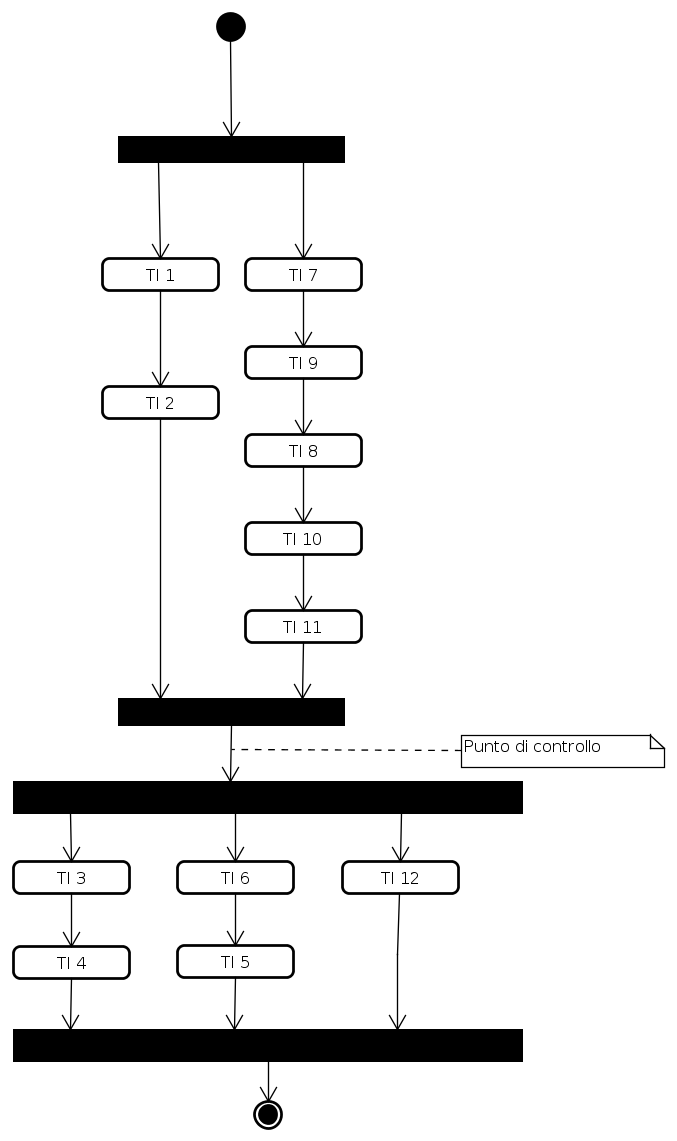
\includegraphics[scale=0.45]{DiagrammaDiAttivita.png}
	\caption{Diagramma di attività dei test di integrazione}
\end{figure}
\FloatBarrier